\subsection{Углы Эйлера}
Пусть у нас имеются некоторый неподвижный базис Oxyz и тело с неподвижной точкой O. В эту точку поместим начало координат системы $\xi\eta\zeta$, в которой все точки тела неподвижны. Эта система жестко связана с телом, поэтому будем считать, что ее ориентация в пространстве относительно  задает ориентацию тела.\\

Тремя плоскими поворотами вокруг осей можно параметризовать ориентацию тела с неподвижной точкой. Рассмотрим подробнее \textbf{углы Эйлера}.
\begin{figure}[!h]
    \centering
    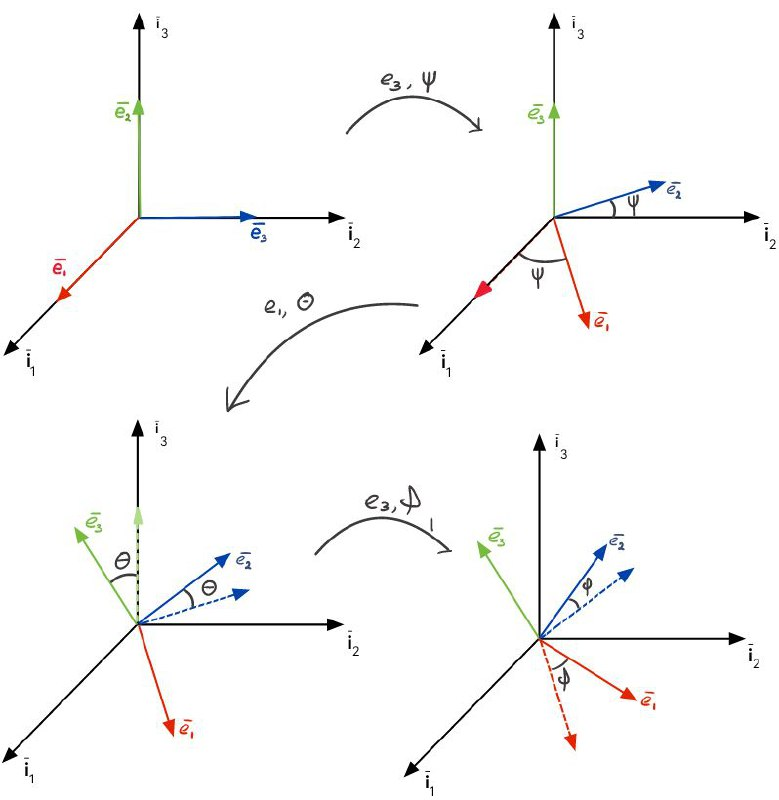
\includegraphics[width=0.75\linewidth]{images/лекция_5_1.jpeg}
\end{figure}
Первый поворот осуществляется на угол $\psi$ (угол прецессии) вокруг оси $e_3$, второй --- на угол $\Theta$ (угол нутации) вокруг $e_1$ и третий --- на угол $\phi$ (угол собственного вращения) вокруг $e_3$. Также последовательность поворотов можно задавать номерами осей, относительно которых происходит вращение, так, для углов Эйлера получим 3-1-3.\\

Углы Эйлера --- одна из последовательностей поворотов, входящих в \textbf{систему углов конечного вращения}:
\[
1-2-3 \tab 3-1-2 \tab 2-3-1
\]
\[
1-3-2 \tab 3-2-1 \tab 2-1-3
\]
\[
1-2-1 \tab 2-3-2 \tab 3-1-3
\]
\[
1-3-1 \tab 2-1-2 \tab 3-2-3
\]
Первые две строчки --- углы конечного вращения первого рода, последние две --- второго рода.\\
\newpage
\begin{frame}{Фан факт}\\
    Пример с самолетом.
    \begin{figure}[!h]
        \centering
        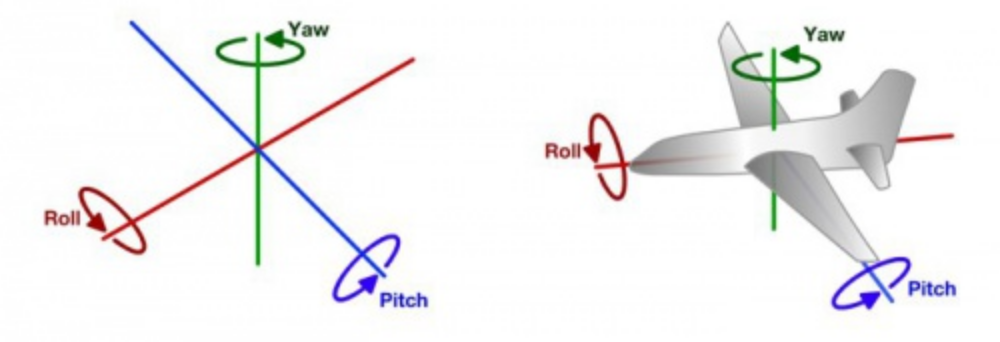
\includegraphics[width=0.75\linewidth]{images/лекция_5_3.png}
    \end{figure}
\end{frame}

\subsubsection{Кинематические уравнения в углах Эйлера}
\textbf{Кинематическими уравнениями} вращательного движения твердого тела называются уравнения, связывающие в дифференциальной форме переменные, ориентацию твердого тела, с угловой скоростью твердого тела. Выведем их, используя углы Эйлера.\\

Движение тела представляет собой сумму трех вращений:
\[
(e_3, \psi) \tab u_3(\psi) = \begin{pmatrix}
    \cos{\psi} & -\sin{\psi} & 0 \\
    \sin{\psi} & \cos{\psi} & 0 \\
    0 & 0 & 1\\
\end{pmatrix}^T
\]
\[
(e_1, \Theta) \tab u_1(\Theta) = \begin{pmatrix}
    1 & 0 & 0\\
    0 & \cos{\Theta} & -\sin{\Theta}\\
    0 & \sin{\Theta} & \cos{\Theta}\\
\end{pmatrix}^T
\]
\[
(e_3, \phi) \tab u_3(\phi) = \begin{pmatrix}
    \cos{\phi} & -\sin{\phi} & 0 \\
    \sin{\phi} & \cos{\phi} & 0 \\
    0 & 0 & 1\\
\end{pmatrix}^T
\]
Используя формулу сложения угловых скоростей, получим $\vec{\omega} = (p~q~r)^T$, где p, q, r --- координаты разложения угловой скорости в собственных осях $(e_1, e_2, e_3)$: 
\[
\begin{pmatrix}
    p\\
    q\\
    r\\
\end{pmatrix} = \begin{pmatrix}
    0\\
    0\\
    \dot{\phi}\\ 
\end{pmatrix} + u_3(\phi)\begin{pmatrix}
    \dot{\Theta}\\
    0\\
    0\\
\end{pmatrix} + u_1(\Theta) u_3(\phi)\begin{pmatrix}
    0\\
    0\\
    \dot{\psi}\\
\end{pmatrix} \Longrightarrow
\]
\[
\begin{cases}
    p = \dot{\Theta} \cos{\phi} + \dot{\psi}\sin{\Theta}\sin{\phi}\\
    q = -\dot{\Theta} \sin{\phi} + \dot{\psi}\sin{\Theta}\cos{\phi}\\
    r = \dot{\phi} + \dot{\psi}\cos{\Theta}\\
\end{cases}
\]
\hypertarget{kinematic_Euler_equations}{}
Или же \textbf{кинематические уравнения Эйлера}:
\[
\begin{cases}
    \dot{\psi} = \dfrac{p \sin{\phi} + q \cos{\phi}}{\sin{\Theta}}\\
    \dot{\phi} = r - ctg~{\Theta} \cdot (p \sin{\phi} + q \cos{\phi})\\
    \dot{\Theta} = p \cos{\phi} - q \sin{\phi}\\
\end{cases}
\]


\section{Динамика}
\subsection{Основные понятия}
В этом разделе рассматриваются системы материальных точек, основное используемое уравнение --- второй закон Ньютона.\\

На точки в системе действуют силы, они разделяются на \textbf{внешние} и \textbf{внутренние}, т.е. что-то, что действует со стороны других тел, и что-то, действующее изнутри соответственно.\\

К основным динамическим характеристикам тела относятся \textbf{импульс}, \textbf{кинетический момент} и \textbf{кинетическая энергия}. Введем эти и некоторые другие величины.\\

Импульс или количество движения:
\[
\vec{p} = m\vec{v} \tab \vec{p} = \sum m_i\vec{v}_i = \int\limits_S\vec{v}~dm
\]
Кинетический момент или момент импульса относительно полюса $A$:
\[
\vec{K}_A = \sum \vec{r}_{A_i} \times m_i\vec{v}_i
\]
Центр масс:
\[
\vec{r}_C = \dfrac{\sum \vec{r}_im_i}{\sum m_i}
\]
Импульс силы:
\[
I = \int\limits_{t_1}^{t_2} F~d t
\]
Мощность силы:
\[
N = \vec{F} \cdot \vec{v}
\]
Работа силы:
\[
\delta A = \vec{F} \cdot \vec{v}~ dt \tab A = \int\limits_{t_1}^{t_2} \vec{F} \cdot \vec{v}~d t
\]
Кинетическая энергия:
\[
T = \dfrac{1}{2}\sum m_i\vec{v}_i \cdot \vec{v_i}
\]